
\usepackage{amsfonts}
\usepackage{amsmath}
\usepackage{amssymb}

\usepackage{graphicx}

\usepackage{fancyhdr}
\usepackage{dsfont}

\usepackage{rotating}
\usepackage{shortvrb}
\usepackage{multicol}
\usepackage{longtable}
\usepackage{xr}

\usepackage{thumbpdf}
\usepackage{hyperref}
\usepackage{xspace}

\input{prepictex}
\input{pictexwd}
\input{postpictex}

\usepackage[dcu]{harvard}

\hypersetup{
    pdfstartview=FitB,
    pdftitle={BayesX Manuals},
    pdfauthor={Christiane Belitz, Andreas Brezger, Nadja Klein, Thomas Kneib, Stefan Lang and Nikolaus Umlauf},
    colorlinks=true,
    linkcolor=blue,
    pdfpagemode=UseOutlines,
    bookmarksopen=true,
    bookmarksnumbered=true,
    pdfstartpage={1},
    hyperindex=true
    }


 \sloppy
 \setlength{\parindent}{0cm}
 \setlength{\parskip}{0.3em}

 \setlength{\paperheight}{29.7cm}
 \setlength{\paperwidth}{20.5cm}

 \setlength{\textheight}{24cm}
 \setlength{\textwidth}{16.5cm}
 \setlength{\headheight}{0.5cm}

 \setlength{\topmargin}{-0.3cm}
 \setlength{\oddsidemargin}{-0.4cm}
 \setlength{\evensidemargin}{-0.4cm}

 \renewcommand{\baselinestretch}{1.0}
 
 \fancyhead[RO,LE]{\thepage}
 \fancyhead[C]{}
 \fancyhead[LO]{\nouppercase\rightmark}
 \fancyhead[RE]{\nouppercase\leftmark}
 \fancyfoot[RO,LE]{}
 \fancyfoot[LO,RE]{}
 \fancyfoot[C]{}

 \pagestyle{fancy}

 \renewcommand{\headrulewidth}{.4pt}
 \renewcommand{\footrulewidth}{0pt}

\newcommand{\BayesX}{\emph{BayesX}\xspace}

\DeclareMathOperator{\Cov}{\mbox{Cov}}
\DeclareMathOperator{\diag}{\mbox{diag}}
\DeclareMathOperator{\trace}{\mbox{trace}}
\DeclareMathOperator{\df}{\mbox{df}}

\def \avec {\text{\boldmath$a$}}    \def \mA {\text{\boldmath$A$}}
\def \bvec {\text{\boldmath$b$}}    \def \mB {\text{\boldmath$B$}}
\def \cvec {\text{\boldmath$c$}}    \def \mC {\text{\boldmath$C$}}
\def \dvec {\text{\boldmath$d$}}    \def \mD {\text{\boldmath$D$}}
\def \evec {\text{\boldmath$e$}}    \def \mE {\text{\boldmath$E$}}
\def \fvec {\text{\boldmath$f$}}    \def \mF {\text{\boldmath$F$}}
\def \gvec {\text{\boldmath$g$}}    \def \mG {\text{\boldmath$G$}}
\def \hvec {\text{\boldmath$h$}}    \def \mH {\text{\boldmath$H$}}
\def \ivec {\text{\boldmath$i$}}    \def \mI {\text{\boldmath$I$}}
\def \jvec {\text{\boldmath$j$}}    \def \mJ {\text{\boldmath$J$}}
\def \kvec {\text{\boldmath$k$}}    \def \mK {\text{\boldmath$K$}}
\def \lvec {\text{\boldmath$l$}}    \def \mL {\text{\boldmath$L$}}
\def \mvec {\text{\boldmath$m$}}    \def \mM {\text{\boldmath$M$}}
\def \nvec {\text{\boldmath$n$}}    \def \mN {\text{\boldmath$N$}}
\def \ovec {\text{\boldmath$o$}}    \def \mO {\text{\boldmath$O$}}
\def \pvec {\text{\boldmath$p$}}    \def \mP {\text{\boldmath$P$}}
\def \qvec {\text{\boldmath$q$}}    \def \mQ {\text{\boldmath$Q$}}
\def \rvec {\text{\boldmath$r$}}    \def \mR {\text{\boldmath$R$}}
\def \svec {\text{\boldmath$s$}}    \def \mS {\text{\boldmath$S$}}
\def \tvec {\text{\boldmath$t$}}    \def \mT {\text{\boldmath$T$}}
\def \uvec {\text{\boldmath$u$}}    \def \mU {\text{\boldmath$U$}}
\def \vvec {\text{\boldmath$v$}}    \def \mV {\text{\boldmath$V$}}
\def \wvec {\text{\boldmath$w$}}    \def \mW {\text{\boldmath$W$}}
\def \xvec {\text{\boldmath$x$}}    \def \mX {\text{\boldmath$X$}}
\def \yvec {\text{\boldmath$y$}}    \def \mY {\text{\boldmath$Y$}}
\def \zvec {\text{\boldmath$z$}}    \def \mZ {\text{\boldmath$Z$}}
\def \nuvec {\text{\boldmath$\nu$}}

\def \ahatvec {\text{\boldmath$\hat a$}}    \def \mhatA {\text{\boldmath$\hat A$}}
\def \bhatvec {\text{\boldmath$\hat b$}}    \def \mhatB {\text{\boldmath$\hat B$}}
\def \chatvec {\text{\boldmath$\hat c$}}    \def \mhatC {\text{\boldmath$\hat C$}}
\def \dhatvec {\text{\boldmath$\hat d$}}    \def \mhatD {\text{\boldmath$\hat D$}}
\def \ehatvec {\text{\boldmath$\hat e$}}    \def \mhatE {\text{\boldmath$\hat E$}}
\def \fhatvec {\text{\boldmath$\hat f$}}    \def \mhatF {\text{\boldmath$\hat F$}}
\def \ghatvec {\text{\boldmath$\hat g$}}    \def \mhatG {\text{\boldmath$\hat G$}}
\def \hhatvec {\text{\boldmath$\hat h$}}    \def \mhatH {\text{\boldmath$\hat H$}}
\def \ihatvec {\text{\boldmath$\hat i$}}    \def \mhatI {\text{\boldmath$\hat I$}}
\def \jhatvec {\text{\boldmath$\hat j$}}    \def \mhatJ {\text{\boldmath$\hat J$}}
\def \khatvec {\text{\boldmath$\hat k$}}    \def \mhatK {\text{\boldmath$\hat K$}}
\def \lhatvec {\text{\boldmath$\hat l$}}    \def \mhatL {\text{\boldmath$\hat L$}}
\def \mhatvec {\text{\boldmath$\hat m$}}    \def \mhatM {\text{\boldmath$\hat M$}}
\def \nhatvec {\text{\boldmath$\hat n$}}    \def \mhatN {\text{\boldmath$\hat N$}}
\def \ohatvec {\text{\boldmath$\hat o$}}    \def \mhatO {\text{\boldmath$\hat O$}}
\def \phatvec {\text{\boldmath$\hat p$}}    \def \mhatP {\text{\boldmath$\hat P$}}
\def \qhatvec {\text{\boldmath$\hat q$}}    \def \mhatQ {\text{\boldmath$\hat Q$}}
\def \rhatvec {\text{\boldmath$\hat r$}}    \def \mhatR {\text{\boldmath$\hat R$}}
\def \shatvec {\text{\boldmath$\hat s$}}    \def \mhatS {\text{\boldmath$\hat S$}}
\def \thatvec {\text{\boldmath$\hat t$}}    \def \mhatT {\text{\boldmath$\hat T$}}
\def \uhatvec {\text{\boldmath$\hat u$}}    \def \mhatU {\text{\boldmath$\hat U$}}
\def \vhatvec {\text{\boldmath$\hat v$}}    \def \mhatV {\text{\boldmath$\hat V$}}
\def \whatvec {\text{\boldmath$\hat w$}}    \def \mhatW {\text{\boldmath$\hat W$}}
\def \xhatvec {\text{\boldmath$\hat x$}}    \def \mhatX {\text{\boldmath$\hat X$}}
\def \yhatvec {\text{\boldmath$\hat y$}}    \def \mhatY {\text{\boldmath$\hat Y$}}
\def \zhatvec {\text{\boldmath$\hat z$}}    \def \mhatZ {\text{\boldmath$\hat Z$}}

\def \abarvec {\text{\boldmath$\bar a$}}    \def \mbarA {\text{\boldmath$\bar A$}}
\def \bbarvec {\text{\boldmath$\bar b$}}    \def \mbarB {\text{\boldmath$\bar B$}}
\def \cbarvec {\text{\boldmath$\bar c$}}    \def \mbarC {\text{\boldmath$\bar C$}}
\def \dbarvec {\text{\boldmath$\bar d$}}    \def \mbarD {\text{\boldmath$\bar D$}}
\def \ebarvec {\text{\boldmath$\bar e$}}    \def \mbarE {\text{\boldmath$\bar E$}}
\def \fbarvec {\text{\boldmath$\bar f$}}    \def \mbarF {\text{\boldmath$\bar F$}}
\def \gbarvec {\text{\boldmath$\bar g$}}    \def \mbarG {\text{\boldmath$\bar G$}}
\def \hbarvec {\text{\boldmath$\bar h$}}    \def \mbarH {\text{\boldmath$\bar H$}}
\def \ibarvec {\text{\boldmath$\bar i$}}    \def \mbarI {\text{\boldmath$\bar I$}}
\def \jbarvec {\text{\boldmath$\bar j$}}    \def \mbarJ {\text{\boldmath$\bar J$}}
\def \kbarvec {\text{\boldmath$\bar k$}}    \def \mbarK {\text{\boldmath$\bar K$}}
\def \lbarvec {\text{\boldmath$\bar l$}}    \def \mbarL {\text{\boldmath$\bar L$}}
\def \mbarvec {\text{\boldmath$\bar m$}}    \def \mbarM {\text{\boldmath$\bar M$}}
\def \nbarvec {\text{\boldmath$\bar n$}}    \def \mbarN {\text{\boldmath$\bar N$}}
\def \obarvec {\text{\boldmath$\bar o$}}    \def \mbarO {\text{\boldmath$\bar O$}}
\def \pbarvec {\text{\boldmath$\bar p$}}    \def \mbarP {\text{\boldmath$\bar P$}}
\def \qbarvec {\text{\boldmath$\bar q$}}    \def \mbarQ {\text{\boldmath$\bar Q$}}
\def \rbarvec {\text{\boldmath$\bar r$}}    \def \mbarR {\text{\boldmath$\bar R$}}
\def \sbarvec {\text{\boldmath$\bar s$}}    \def \mbarS {\text{\boldmath$\bar S$}}
\def \tbarvec {\text{\boldmath$\bar t$}}    \def \mbarT {\text{\boldmath$\bar T$}}
\def \ubarvec {\text{\boldmath$\bar u$}}    \def \mbarU {\text{\boldmath$\bar U$}}
\def \vbarvec {\text{\boldmath$\bar v$}}    \def \mbarV {\text{\boldmath$\bar V$}}
\def \wbarvec {\text{\boldmath$\bar w$}}    \def \mbarW {\text{\boldmath$\bar W$}}
\def \xbarvec {\text{\boldmath$\bar x$}}    \def \mbarX {\text{\boldmath$\bar X$}}
\def \ybarvec {\text{\boldmath$\bar y$}}    \def \mbarY {\text{\boldmath$\bar Y$}}
\def \zbarvec {\text{\boldmath$\bar z$}}    \def \mbarZ {\text{\boldmath$\bar Z$}}

\def \atildevec {\text{\boldmath$\tilde a$}}    \def \mtildeA {\text{\boldmath$\tilde A$}}
\def \btildevec {\text{\boldmath$\tilde b$}}    \def \mtildeB {\text{\boldmath$\tilde B$}}
\def \ctildevec {\text{\boldmath$\tilde c$}}    \def \mtildeC {\text{\boldmath$\tilde C$}}
\def \dtildevec {\text{\boldmath$\tilde d$}}    \def \mtildeD {\text{\boldmath$\tilde D$}}
\def \etildevec {\text{\boldmath$\tilde e$}}    \def \mtildeE {\text{\boldmath$\tilde E$}}
\def \ftildevec {\text{\boldmath$\tilde f$}}    \def \mtildeF {\text{\boldmath$\tilde F$}}
\def \gtildevec {\text{\boldmath$\tilde g$}}    \def \mtildeG {\text{\boldmath$\tilde G$}}
\def \htildevec {\text{\boldmath$\tilde h$}}    \def \mtildeH {\text{\boldmath$\tilde H$}}
\def \itildevec {\text{\boldmath$\tilde i$}}    \def \mtildeI {\text{\boldmath$\tilde I$}}
\def \jtildevec {\text{\boldmath$\tilde j$}}    \def \mtildeJ {\text{\boldmath$\tilde J$}}
\def \ktildevec {\text{\boldmath$\tilde k$}}    \def \mtildeK {\text{\boldmath$\tilde K$}}
\def \ltildevec {\text{\boldmath$\tilde l$}}    \def \mtildeL {\text{\boldmath$\tilde L$}}
\def \mtildevec {\text{\boldmath$\tilde m$}}    \def \mtildeM {\text{\boldmath$\tilde M$}}
\def \ntildevec {\text{\boldmath$\tilde n$}}    \def \mtildeN {\text{\boldmath$\tilde N$}}
\def \otildevec {\text{\boldmath$\tilde o$}}    \def \mtildeO {\text{\boldmath$\tilde O$}}
\def \ptildevec {\text{\boldmath$\tilde p$}}    \def \mtildeP {\text{\boldmath$\tilde P$}}
\def \qtildevec {\text{\boldmath$\tilde q$}}    \def \mtildeQ {\text{\boldmath$\tilde Q$}}
\def \rtildevec {\text{\boldmath$\tilde r$}}    \def \mtildeR {\text{\boldmath$\tilde R$}}
\def \stildevec {\text{\boldmath$\tilde s$}}    \def \mtildeS {\text{\boldmath$\tilde S$}}
\def \ttildevec {\text{\boldmath$\tilde t$}}    \def \mtildeT {\text{\boldmath$\tilde T$}}
\def \utildevec {\text{\boldmath$\tilde u$}}    \def \mtildeU {\text{\boldmath$\tilde U$}}
\def \vtildevec {\text{\boldmath$\tilde v$}}    \def \mtildeV {\text{\boldmath$\tilde V$}}
\def \wtildevec {\text{\boldmath$\tilde w$}}    \def \mtildeW {\text{\boldmath$\tilde W$}}
\def \xtildevec {\text{\boldmath$\tilde x$}}    \def \mtildeX {\text{\boldmath$\tilde X$}}
\def \ytildevec {\text{\boldmath$\tilde y$}}    \def \mtildeY {\text{\boldmath$\tilde Y$}}
\def \ztildevec {\text{\boldmath$\tilde z$}}    \def \mtildeZ {\text{\boldmath$\tilde Z$}}

\def \alphavec        {\text{\boldmath$\alpha$}}
\def \betavec         {\text{\boldmath$\beta$}}
\def \gammavec        {\text{\boldmath$\gamma$}}
\def \deltavec        {\text{\boldmath$\delta$}}
\def \epsilonvec      {\text{\boldmath$\epsilon$}}
\def \varepsilonvec   {\text{\boldmath$\varepsilon$}}
\def \zetavec         {\text{\boldmath$\zeta$}}
\def \etavec          {\text{\boldmath$\eta$}}
\def \thetavec        {\text{\boldmath$\theta$}}
\def \varthetavec     {\text{\boldmath$\vartheta$}}
\def \iotavec         {\text{\boldmath$\iota$}}
\def \kappavec        {\text{\boldmath$\kappa$}}
\def \lambdavec       {\text{\boldmath$\lambda$}}
\def \muvec           {\text{\boldmath$\mu$}}
\def \nuvec           {\text{\boldmath$\nu$}}
\def \xivec           {\text{\boldmath$\xi$}}
\def \pivec           {\text{\boldmath$\pi$}}
\def \varpivec        {\text{\boldmath$\varpi$}}
\def \rhovec          {\text{\boldmath$\rho$}}
\def \varrhovec       {\text{\boldmath$\varrho$}}
\def \sigmavec        {\text{\boldmath$\sigma$}}
\def \varsigmavec     {\text{\boldmath$\varsigma$}}
\def \tauvec          {\text{\boldmath$\tau$}}
\def \upsilonvec      {\text{\boldmath$\upsilon$}}
\def \phivec          {\text{\boldmath$\phi$}}
\def \varphivec       {\text{\boldmath$\varphi$}}
\def \psivec          {\text{\boldmath$\psi$}}
\def \chivec          {\text{\boldmath$\chi$}}
\def \omegavec        {\text{\boldmath$\omega$}}

\def \alphahatvec        {\text{\boldmath$\hat \alpha$}}
\def \betahatvec         {\text{\boldmath$\hat \beta$}}
\def \betahathatvec      {\text{\boldmath$\hat{\hat\beta}$}}
\def \gammahatvec        {\text{\boldmath$\hat \gamma$}}
\def \deltahatvec        {\text{\boldmath$\hat \delta$}}
\def \epsilonhatvec      {\text{\boldmath$\hat \epsilon$}}
\def \varepsilonhatvec   {\text{\boldmath$\hat \varepsilon$}}
\def \varepsilonhathatvec{\text{\boldmath$\hat{\hat\varepsilon}$}}
\def \zetahatvec         {\text{\boldmath$\hat \zeta$}}
\def \etahatvec          {\text{\boldmath$\hat \eta$}}
\def \thetahatvec        {\text{\boldmath$\hat \theta$}}
\def \varthetahatvec     {\text{\boldmath$\hat \vartheta$}}
\def \iotahatvec         {\text{\boldmath$\hat \iota$}}
\def \kappahatvec        {\text{\boldmath$\hat \kappa$}}
\def \lambdahatvec       {\text{\boldmath$\hat \lambda$}}
\def \muhatvec           {\text{\boldmath$\hat \mu$}}
\def \nuhatvec           {\text{\boldmath$\hat \nu$}}
\def \xihatvec           {\text{\boldmath$\hat \xi$}}
\def \pihatvec           {\text{\boldmath$\hat \pi$}}
\def \varpihatvec        {\text{\boldmath$\hat \varpi$}}
\def \rhohatvec          {\text{\boldmath$\hat \rho$}}
\def \varrhohatvec       {\text{\boldmath$\hat \varrho$}}
\def \sigmahatvec        {\text{\boldmath$\hat \sigma$}}
\def \varsigmahatvec     {\text{\boldmath$\hat \varsigma$}}
\def \tauhatvec          {\text{\boldmath$\hat \tau$}}
\def \upsilonhatvec      {\text{\boldmath$\hat \upsilon$}}
\def \phihatvec          {\text{\boldmath$\hat \phi$}}
\def \varphihatvec       {\text{\boldmath$\hat \varphi$}}
\def \psihatvec          {\text{\boldmath$\hat \psi$}}
\def \chihatvec          {\text{\boldmath$\hat \chi$}}
\def \omegahatvec        {\text{\boldmath$\hat \omega$}}

\def \alphatildevec        {\text{\boldmath$\tilde \alpha$}}
\def \betatildevec         {\text{\boldmath$\tilde \beta$}}
\def \gammatildevec        {\text{\boldmath$\tilde \gamma$}}
\def \deltatildevec        {\text{\boldmath$\tilde \delta$}}
\def \epsilontildevec      {\text{\boldmath$\tilde \epsilon$}}
\def \varepsilontildevec   {\text{\boldmath$\tilde \varepsilon$}}
\def \zetatildevec         {\text{\boldmath$\tilde \zeta$}}
\def \etatildevec          {\text{\boldmath$\tilde \eta$}}
\def \thetatildevec        {\text{\boldmath$\tilde \theta$}}
\def \varthetatildevec     {\text{\boldmath$\tilde \vartheta$}}
\def \iotatildevec         {\text{\boldmath$\tilde \iota$}}
\def \kappatildevec        {\text{\boldmath$\tilde \kappa$}}
\def \lambdatildevec       {\text{\boldmath$\tilde \lambda$}}
\def \mutildevec           {\text{\boldmath$\tilde \mu$}}
\def \nutildevec           {\text{\boldmath$\tilde \nu$}}
\def \xitildevec           {\text{\boldmath$\tilde \xi$}}
\def \pitildevec           {\text{\boldmath$\tilde \pi$}}
\def \varpitildevec        {\text{\boldmath$\tilde \varpi$}}
\def \rhotildevec          {\text{\boldmath$\tilde \rho$}}
\def \varrhotildevec       {\text{\boldmath$\tilde \varrho$}}
\def \sigmatildevec        {\text{\boldmath$\tilde \sigma$}}
\def \varsigmatildevec     {\text{\boldmath$\tilde \varsigma$}}
\def \tautildevec          {\text{\boldmath$\tilde \tau$}}
\def \upsilontildevec      {\text{\boldmath$\tilde \upsilon$}}
\def \phitildevec          {\text{\boldmath$\tilde \phi$}}
\def \varphitildevec       {\text{\boldmath$\tilde \varphi$}}
\def \psitildevec          {\text{\boldmath$\tilde \psi$}}
\def \chitildevec          {\text{\boldmath$\tilde \chi$}}
\def \omegatildevec        {\text{\boldmath$\tilde \omega$}}

\def \mGamma   {\mathbf{\Gamma}}
\def \mDelta   {\mathbf{\Delta}}
\def \mTheta   {\mathbf{\Theta}}
\def \mLambda  {\mathbf{\Lambda}}
\def \mXi      {\mathbf{\Xi}}
\def \mPi      {\mathbf{\Pi}}
\def \mSigma   {\mathbf{\Sigma}}
\def \mUpsilon {\mathbf{\Upsilon}}
\def \mPhi     {\mathbf{\Phi}}
\def \mPsi     {\mathbf{\Psi}}
\def \mOmega   {\mathbf{\Omega}}

\def \mhatGamma   {\mathbf{\hat \Gamma}}
\def \mhatDelta   {\mathbf{\hat \Delta}}
\def \mhatTheta   {\mathbf{\hat \Theta}}
\def \mhatLambda  {\mathbf{\hat \Lambda}}
\def \mhatXi      {\mathbf{\hat \Xi}}
\def \mhatPi      {\mathbf{\hat \Pi}}
\def \mhatSigma   {\mathbf{\hat \Sigma}}
\def \mhatUpsilon {\mathbf{\hat \Upsilon}}
\def \mhatPhi     {\mathbf{\hat \Phi}}
\def \mhatPsi     {\mathbf{\hat \Psi}}
\def \mhatOmega   {\mathbf{\hat \Omega}}

\def \nullvec {\mathbf{0}}
\def \onevec {\mathbf{1}}

\def \dsP {\text{$\mathds{P}$}}
\def \dsE {\text{$\mathds{E}$}}
\def \dsR {\text{$\mathds{R}$}}
\def \dsN {\text{$\mathds{N}$}}
\def \dsC {\text{$\mathds{C}$}}
\def \dsZ {\text{$\mathds{Z}$}}

\newcommand{\subheader}[1]
 {
 \textsf{\textbf{{\large #1}}}
 }

\newenvironment{stanza}[1]
 {
 \subheader{#1} 
 \begin{itemize} 
 \item[]
 }
 {
 \end{itemize}
 }


\newcommand{\preface}[1]
 {
 \thispagestyle{empty}
    
 \begin{center}
 {\bfseries \em \huge BayesX}

 \vspace{0.5cm}

 {\em \large Software for Bayesian Inference in Structured Additive Regression Models}

 \vspace{0.5cm}

 {\em Version 4.0}

 \vspace{0.5cm}

 \begin{figure}[h]
 \begin{center}
 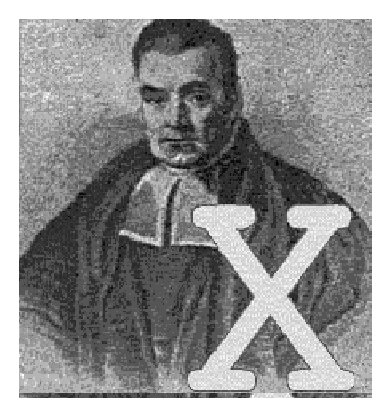
\includegraphics[scale=1.2]{grafiken/bayesicon.eps}
 \end{center}
 \end{figure}

 \vfill

 {\bf\sffamily \huge #1}

 \vfill

 \end{center}

 {\em Developed by}

 Christiane Belitz\\
 Andreas Brezger\\
 Nadja Klein (Humboldt-Universit\"{a}t zu Berlin)\\
 Thomas Kneib (Georg-August-Universit\"{a}t G\"{o}ttingen)\\
 Stefan Lang (University of Innsbruck) \\
 Nikolaus Umlauf (University of Innsbruck) \\

 \vspace{2ex}

 {\em With contributions by}

 \vspace{-1.5ex}

 \begin{multicols}{2}
 Daniel Adler\\
 Paul Cochrane\\
 Jan Fahrenholz\\
 Eva-Maria Fronk\\
 Felix Heinzl\\
 Andrea Hennerfeind\\
 Manuela Hummel\\
 Alexander Jerak\\
 Susanne Konrath\\
 Petra Kragler\\
 Cornelia Oberhauser\\
 Leyre Est\'{\i}baliz Osuna Echavarr\'{\i}a\\
 Daniel Saban\'{e}s Bov\'{e} \\
 Paul Wiemann\\
 Achim Zeileis
 \end{multicols}

 {\em Supported by}

 Ludwig Fahrmeir\\
 Leonhard Held\\
 German Research Foundation (DFG)

 \newpage

 \subsection*{Acknowledgements}

 The development of \BayesX has been financially supported by grants from the German Research Foundation (DFG), Collaborative Research Center 386 ``Statistical Analysis of Discrete Structures''. The first versions of BayesX have been developed while Thomas Kneib and Stefan Lang (and several of the contributors) were working with Ludwig Fahrmeir at the Department of Statistics, Ludwig-Maximilians-Universit\"{a}t M\"{u}nchen.

 Special thanks go to (in alphabetical order of first names):

 {\em Dieter Gollnow} for setting up and providing the map of Munich (a really hard job); \\
 {\em Leonhard Held} for advertising the program; \\
 {\em Ludwig Fahrmeir} for his patience with finishing a first version of the program and for carefully reading and correcting the manual; \\
 {\em Ngianga-Bakwin Kandala} for being the first user of the program (a really hard job); \\
 {\em Samson Babatunde Adebayo} for carefully reading and correcting the manual; \\
 {\em Ursula Becker} for carefully reading and correcting the manual.

 \subsection*{Licensing agreement}

This program is free software; you can redistribute it and/or modify it under the terms of the GNU General Public License
as published by the Free Software Foundation; either version 2 of the License, or (at your option) any later version.

This program is distributed in the hope that it will be useful, but WITHOUT ANY WARRANTY; without even the implied warranty of MERCHANTABILITY or FITNESS FOR A PARTICULAR PURPOSE. See the GNU General Public License for more details.

You should have received a copy of the GNU General Public License along with this program; if not, write to the Free Software Foundation, Inc., 51 Franklin Street, Fifth Floor, Boston, MA  02110-1301, USA.

\vspace{0.5cm}

\BayesX is available at { \href{http://www.bayesx.org}{http://www.bayesx.org}}}
